\documentclass{ueacmpstyle}

\usepackage{natbib}
\usepackage{url}
\usepackage{graphicx}
\usepackage{float}

\title{Team Report: Evolution Sandbox}
\author{Benjamin Longhurst, Rupert Hammond, Ryan Phelan, Travis Payne}

\begin{document}
	
\maketitle

\section{Introduction}
\subsection{Evolution Simulation}
An evolution simulation attempts to represent the way a set of organisms evolve within a limited ecosystem. Typically a number of biological algorithms such as fitness functions and crossover are employed to dictate how this evolution plays out. 

One such example of an evolution simulation is Conway's Game of Life. Created in 1970 by John Conway, the simulation takes place on an infinitely sized grid where each cell can either be live or dead. It progresses according to a set of simple rules [\cite{guardian}]:
\begin{itemize}
	\item A live cell with less than two live neighbours becomes dead
	\item A live cell with more than four live neighbours becomes dead
	\item A dead cell with three live neighbours becomes alive
\end{itemize}

Conway's Game of Life is often praised for its ability to show how simple rules can spawn complex evolutionary patterns [\cite{callahan}]. It was initially considered as a potential starting base for the project due to it's relative simplicity and the fact that the well-defined rules could be painlessly tweaked or switched out as development progressed. However, it was instead used as a more loose inspiration with core ideas such as a grid-based and rule-focused approach influencing the project.

\subsection{Project Overview}
This project aims to produce an evolution sandbox; a simulation with emphasis on real-time manipulation and customization which allows the user to observe the outcome of their actions. The basic requirements are defined as follows:
\begin{itemize}
	\item The simulation should be based on a set of realistic biological algorithms and rules
	\item The organisms' path-finding should be logical
	\item The simulation should be able to handle a large number of organisms without noticeable lag
	\item The organisms' attributes should be customisable on the fly
	\item The ecosystem should reach equilibrium when left to its own devices
	\item The UI should be clean, simple and with a professional feeling
	\item The 2D graphics should faithfully represent the underlying simulation
\end{itemize}

\section{Design}

\subsection{Analysis}

Several analysis' were carried out against the initial requirements to better determine an order of priorities and establish the project scope:

\paragraph{Object Oriented Analysis}
	\begin{itemize}
		\item End Goal: Biological Evolution Sandbox
		\begin{itemize}
			\item What is required?
			\begin{itemize}
				\item End game, stable ecology
					\begin{itemize}
						\item Net number of organisms doesn't change
					\end{itemize}
				\item Food, vegetation, other organisms
				\item Water
					\begin{itemize}
						\item Some organisms can go in water
					\end{itemize}
				\item Weather
					\begin{itemize}
						\item Hot and cold
						\item Different types of weather
					\end{itemize}
				\item Statistics
				\item A log
				\item Disease
				\item Natural Disasters
				\item Terrain
				\item Live edit of organisms
				\item Tile-based graphics
			\end{itemize}
		\end{itemize}
	\end{itemize}

\pagebreak
\paragraph{MoSCoW Analysis}
\begin{center}
	\begin{tabular}{c|p{0.8\textwidth}}
		Must Have & \begin{itemize}
						\item Organism life cycle
						\item Genetic crossover algorithm
						\item Organism attributes
						\item Live edit of organisms
						\item Simple 2D graphics
						\item Herbivores and natural food sources
					\end{itemize} \\ \hline
		Should Have & \begin{itemize}
						\item Weather/disease system
						\item Advanced path-finding algorithm
						\item Carnivores and predator/prey organisms
						\item Terrain variation, e.g. grass, mountainous, water
						\item Ability to pause, speed up and slow down simulation
					\end{itemize} \\ \hline
		Could Have & \begin{itemize}
						\item Natural disasters
						\item Speciation
						\item A game log with charts and text output
						\item Spritesheet animation
						\item Particle effects, e.g. weather effects, running water, blood
					\end{itemize} \\ \hline
		Won't Have & \begin{itemize}
						\item 3D graphics
						\item Scale realism
					\end{itemize} \\
	\end{tabular}
\end{center}

\subsection{Tools}
Three programming languages were considered for the project: C++, C\# and Java. The simulation was identified to have a large dependency on computation due to the fact that there would be upwards of one hundred organisms on screen at any one time and each of them would require state management, path finding and collision detection. For this reason, C++ seemed to be the natural choice due to the speed benefit of dynamic memory management. However, upon further research it was found that C\# had a more diverse set of 2D graphics libraries as C++ libraries were typically focused on 3D rendering. Finally, Java was considered because the bulk of the team's experience was with the language, though because C\# can be used as a drop-in replacement for Java this was seen as another benefit in using C\#.

With the language decided, a comparison was made between several popular 2D graphics libraries, the four main candidates were Microsoft XNA, MonoGame, UltraViolet (UV) and the Simple Fast Media Library (SFML):

\begin{center}
	\begin{tabular}{c|p{0.4\textwidth}|p{0.4\textwidth}}
		Library & Pros & Cons \\ \hline
		Microsoft XNA & \begin{itemize}
			\item Simple and easy to use
			\item Very well documented
			\item Well-used commercially
			\item Supported by Microsoft who also made C\#
		\end{itemize} & \begin{itemize}
			\item Slow and old, based on DirectX9
			\item Deprecated and no longer works in Visual Studio 2015+
			\item Windows only
			\item Closed source
		\end{itemize} \\ \hline
		MonoGame & \begin{itemize}
			\item Based on XNA with the same syntax, all of the XNA documentation is applicable
			\item Multi-platform but requires Xamarin
			\item Open source
			\item Has seen use on commercial games (Stardew Valley, Transistor, Bastion etc.)
		\end{itemize} & \begin{itemize}
			\item Convoluted asset management system
		\end{itemize} \\ \hline
		UV & \begin{itemize}
			\item Has a built in UI framework based on Windows Presentation Foundation (WPF)
			\item Truly multi-platform
			\item Open source
		\end{itemize} & \begin{itemize}
			\item Convoluted asset management system
			\item Limited documentation, small time
			\item Little to no commercial use
		\end{itemize} \\ \hline
		SFML & \begin{itemize}
			\item Very fast, written in C++ but has C\# bindings
			\item Well documented
			\item Some commercial use
			\item Multi-platform but no phone support
			\item Open source
		\end{itemize} & \begin{itemize}
			\item C\# bindings are slightly behind on updates
			\item Examples and documentation are written in C++ and require conv\label{classdiagram}erting
			\item Syntax is not as simple as other frameworks
		\end{itemize} \\
	\end{tabular}
\end{center}

\pagebreak
Taking these points into account, a proof of concept was made using MonoGame with the third party UI library GeonBit.UI. A UI library was chosen because although any 2D graphics framework is capable of rendering UI using sprite assets, one of the project requirements was that the UI look professional and scientific. Additionally, UI elements such as lists and radio buttons were considered a likely necessity and would be difficult with a graphics approach.

\subsection{Proof of Concept}
A proof of concept was made with the chosen technologies before any further planning took place because the team wanted to avoid a situation where the UML modelling and code architecture was planned according to a language or tool that was then realised to be a poor fit for the project. The aim of the proof of concept was to simply draw a number of organisms to the screen using the chosen graphics framework which could be manipulated using a simple placeholder UI.

\begin{figure}[H]
	\caption{Proof of Concept}\label{classdiagram}
	\centering
	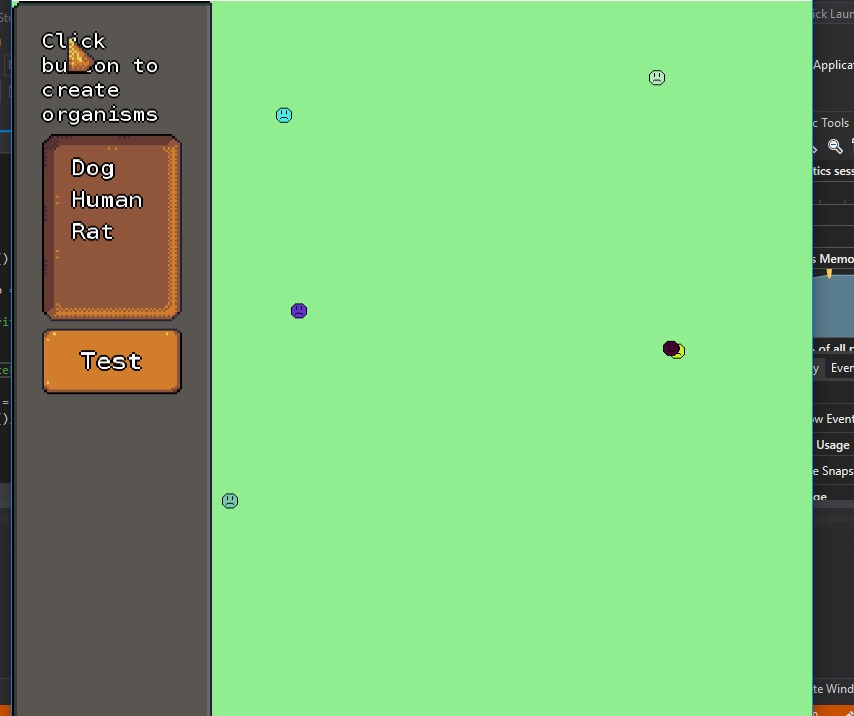
\includegraphics[width=0.8\textwidth]{poc}
\end{figure}

The proof of concept was deemed a success as it was able to create organisms using the UI button, move them around and render them without lag.
\subsection{Modelling}
The class diagram Figure~\ref{classdiagram} was continually updated throughout the project and although it saw many changes, certain key themes remained constant throughout.

An important architectural decision made from the outset was to ensure the separation of concerns between the graphics, simulation and UI. It was decided that the graphical component should provide a representation of the simulation's output, but that they should be kept unaware of the inner workings of the other to better decouple their behaviour. Likewise, while the UI would be able to interact with the simulation, there was no need to have this behaviour tied in any way to the intricacies of it. As such, the relationship between the three key areas can be observed as limited on the class diagram.

Another theme present in the class diagram is abstraction. Through inheritance, MapItems are kept as generic inhabitants by the Tiles of the Grid. This means that the Grid can manage its Tiles and their inhabitant MapItems without particular knowledge of whether they are Organisms, Food or Obstacles, simplifying the implementation.

\section{Project Management}
\subsection{Agile Methodology}
The project is managed according to the Agile methodology, specifically Scrum. Since the code repository is hosted on GitHub, it is used as the project management centre using a combination of it's project boards as seen in Figure~\ref{gitboard} and it's issue tracking from Figure~\ref{gitissue}. Other project management tools include OneNote for collaborative documentation and WhatsApp for quick discussion.

\begin{figure}[H]
	\caption{GitHub Project Board}\label{gitboard}
	\centering
	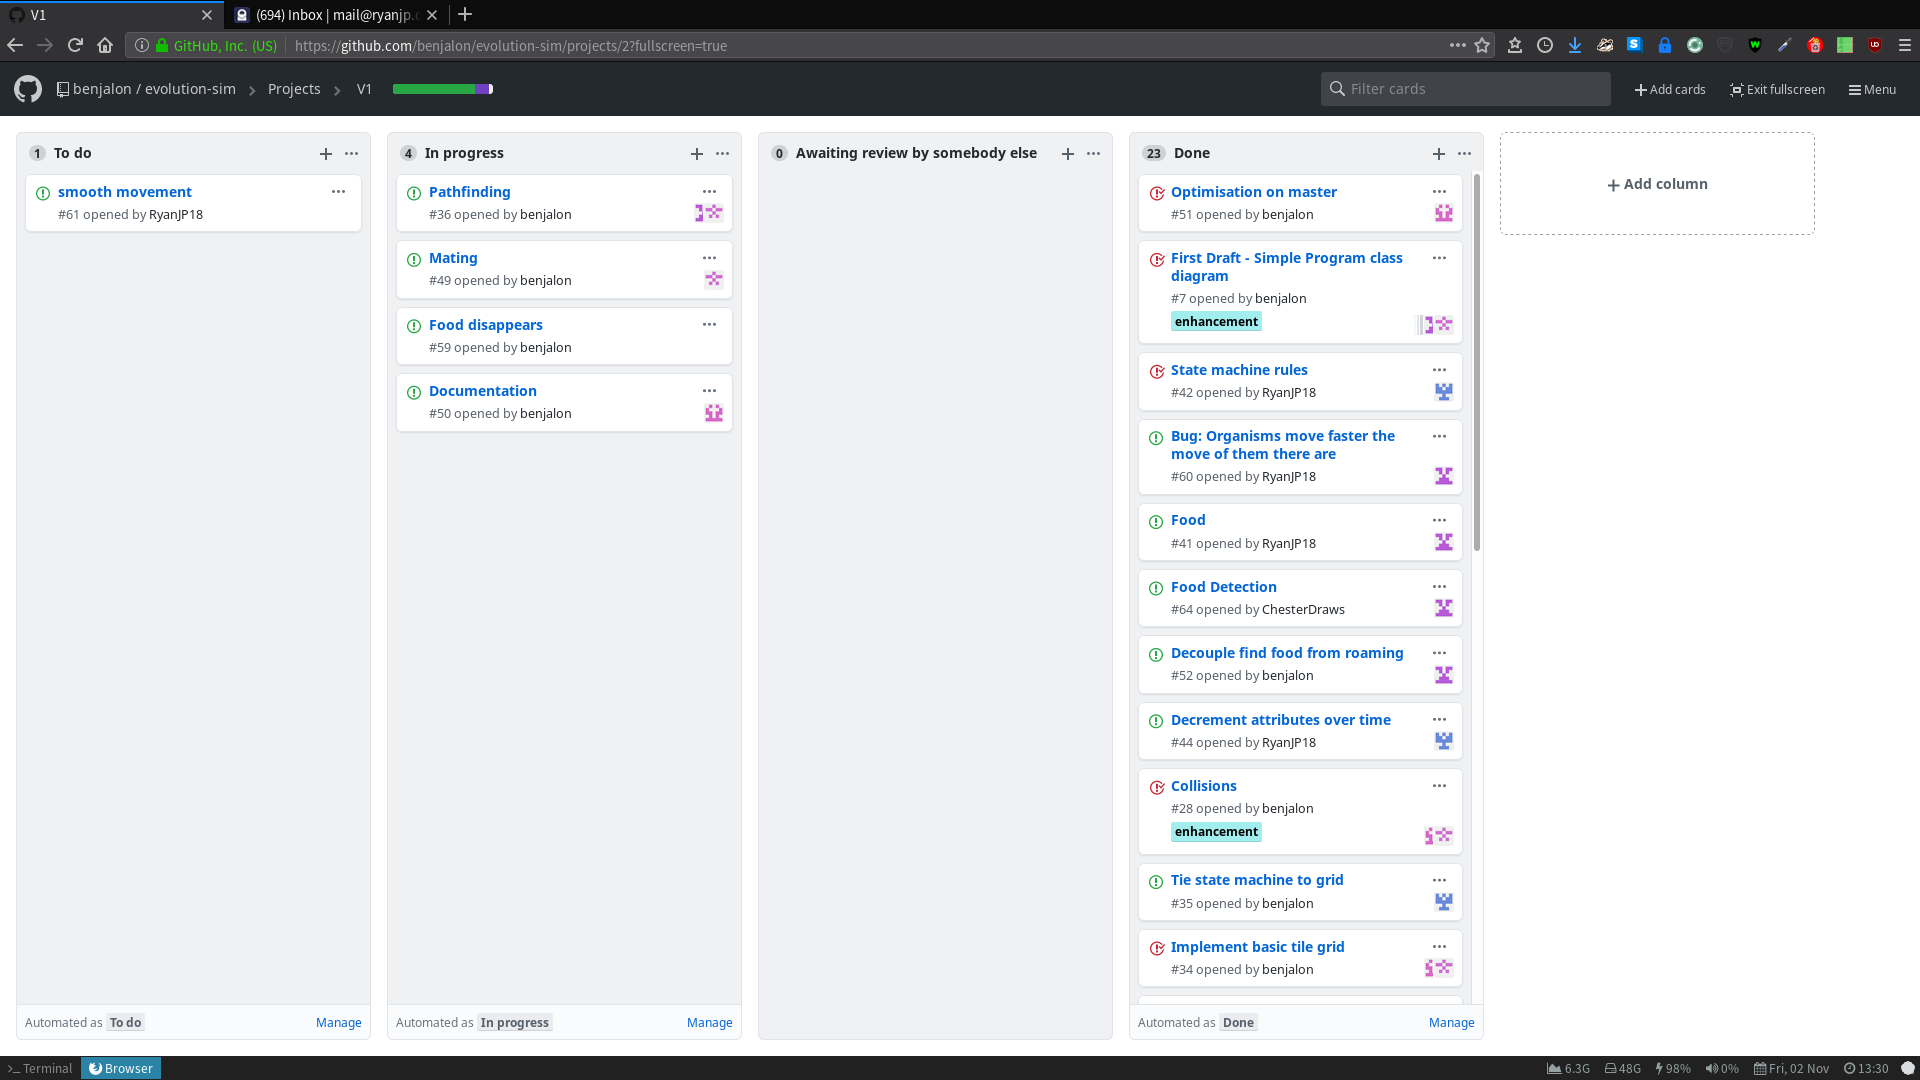
\includegraphics[width=0.8\textwidth]{gitproj}
\end{figure}

\begin{figure}[H]
	\caption{GitHub Issue Tracking}\label{gitissue}
	\centering
	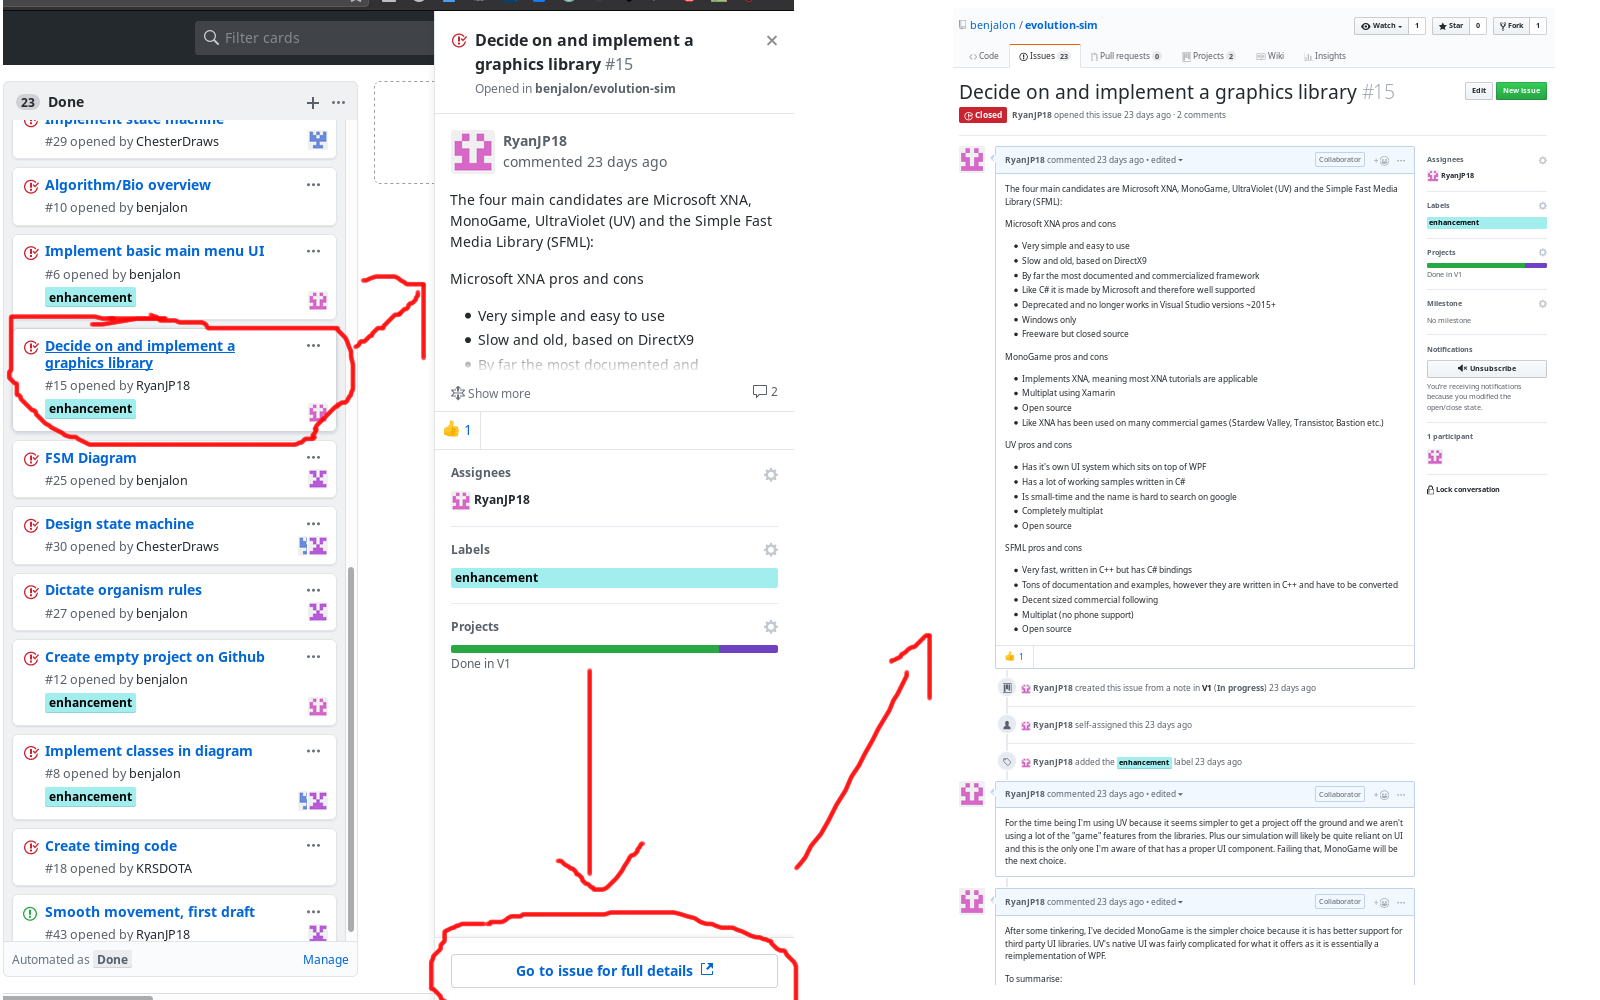
\includegraphics[width=0.8\textwidth]{gitissuetrack}
\end{figure}

Meetings occur twice per week, with one of them being the scheduled lab session. In keeping with the Agile methodology, the iterative releases are promoted with the rule that each lab meeting must have a fully-merged and bug-free master branch. 
Development is split into two to three week sprints, where each of them is contained within a separate project board. This means that any given time, the active project board corresponds to the major release version, which is explained in better detail in Section~\ref{versioning}.  Each meeting begins with a stand-up meeting where each member gives a brief progress report and the team then discuss and realign objectives to meet the end of sprint deadline.

\subsection{Versioning}\label{versioning}
Each sprint begins with a planning meeting where issues are created against the MoSCoW analysis.

	\begin{tabular}{c|p{0.7\textwidth}|l}
		Version & Goal & Deadline \\ \hline
		0 & A proof of concept to test the chosen technologies & Tuesday week 2 \\ \hline
		1 & A fully functioning basic simulation with all of the "must have" components from the MoSCoW analysis & Friday week 6 \\ \hline
		2 & Improvements on V1 simulation with tasks taken from the "should have" objectives. In particular, an advanced path finding algorithm such as A*, improved crossover algorithm, carnivores and a better time system. & Not set\\ \hline
		3+ & TODO & TODO \
	\end{tabular}
		
The logic behind such an approach is that once the base systems are in place, the simulation has a solid foundation can be steadily iterated upon without chance of some areas being left underdeveloped or buggy.
ss
\section{Advanced Programming Concepts}

\subsection{Code Architecture and Practice}
The SOLID principles define five guidelines to code more maintainable and easy to understand [\cite{kelmendi}]: 
\begin{itemize}
	\item Single Responsibility: Every class should have only one responsibility to prevent the class being susceptible to requirement changes.
	\item Open-Closed: Classes should be open to extension but abstraction should be used to avoid the need for rewrites on the extended code.
	\item Liskov Substitution: Derived and base classes should be substitutable.
	\item Interface Segregation: Keep interfaces simple to avoid bulk from implementing unnecessary properties.
	\item Dependency Inversion: Keep abstract code abstract by avoiding dependencies on low level code.
\end{itemize}

While these principles each affect the architecture in some way, in particular a great deal of effort is made to ensure that each class has a single responsibility. An example of this is in separating the Grid from the StateMachine despite the fact that they operate on similar areas of code. The Grid is used as the "graphical brain", positioning organisms and drawing them at their positions, whereas the StateMachine is used as the "logical brain", dictating the behaviour which causes the organisms to be repositioned in the first place. Furthermore, the use of MapItem as a swappable base for Organism and Food would not work if the Liskov Substitution principle was not applied.

To ensure a clean and consistent code-base, the official Microsoft C\# conventions are applied where possible. Notable examples include placing braces on a new line, using camelCase for variable names and avoiding one line if statements [\cite{microsoft}].

\subsection{Grid System}
TODO: might be an unnecessary section but weigh up unrestricted movement vs tile based movement

\subsection{State Management}
TODO someone with more knowledge should write this, for now i've copied what i could find on state management and pasted it in
Organism Behaviour – First Draft

1) Default organism state is “Roaming”.
a. From roaming, an organism can transition to “Seeking Food” or “Seeking Mate”.
2) If an organism is seeking food, it is simply roaming, with the added fact that if it is within a certain range of food, it will go towards it and consume it.
3) If an organism is seeking a mate, it is simply roaming, with the added fact that if it is within a certain range of a mate WHO IS ALSO SEEKING A MATE, it will go towards it and mate.
a. If whilst “Seeking Mate”, the organism becomes Hungry, it will transition to “Seeking Food”. End Goal: Biological Evolution Sandbox
b. What do we want?
i. End game, stable ecology
1. Net number of organisms don’t change
ii. Food, vegetation, other organisms
iii. Water
1. Some organisms can go in water
iv. Weatherdo not need to handle such specific details
1. Hot cold
2. Types of weather
v. Statistics
vi. A log
vii. Dis3ease
viii. Natural Disaster
ix. Terrain
x. Live Edit of organisms
c. Tile based graphicsOnce it has eaten sufficiently, it will go back to default state of roaming.

\subsection{Path Finding Algorithm}
TODO someone with more knowledge should write this.

Simple vs Djkfdshfkdsk's algorithm vs A* algorithm and the benefits of using A*

Should have some references
\subsection{Crossover Algorithm}
TODO someone with more knowledge should write this, should have some references
\subsection{Optimisation}\label{optim}
Optimisation is considered an area of importance due to the simulation's requirement in handling a large number of organisms without noticeable lag. By default, MonoGame's render loop calls two methods at a speed of sixty times per second: update and draw. Should the logic fail to complete within this ~16-17ms time-frame then it delays the draw call, which lowers the simulation's frame-rate. This has further knock-on effects where the draw calls become progressively more delayed and eventually cause input lag on the UI.

The update method is essentially the primary path through the code and handles all of the computation and organism logic. This method calls into several for loops to cycle through the various organisms and map items which make up the simulation. There can be several hundred objects to iterate through during any given Update loop, which as previously mentioned occurs sixty times per second. Keeping this entire iteration within the acceptable ~16-17ms time limit has requires consideration from an optimisation perspective.

To improve the performance of these loops the standard loop optimisations are applied. There are no variables declared within them, collection length is cached locally ahead of time and high precision calculations are also avoided. For example, the DateTime object was initially used to time organism movements but because it uses double precision values, calculations were causing a large slowdown so it was swapped for the better optimised GameTime object. Finally, the grid stores its tiles within a two dimensional array, which can be implemented in C\# in two different ways: multi-dimensional arrays and jagged arrays. A jagged array is an array of arrays and allows these arrays to vary in lengths, whereas a multi-dimensional is a natural 2D array where all of them must all be the same length. The grid stores its tiles in a jagged array because within a jagged array, even if the arrays are the same length, it is able to iterate faster than a multi-dimensional array.

Finally, from an architecture perspective the grid system is also a form of optimisation. By constricting organism movements to a grid the simulation is able to cut down on the need for collision detection by having organisms request their moves to the grid, which then makes the decision of whether the move is legal. Collision detection would otherwise have been a bottleneck for the system which would have been exponentially slower as more organisms are added because each organism would need to check the position all of the others. With other simulation items such as food this becomes more complicated.

\section{Product}

\subsection{Roadmap}

TODO: break down what we did and when

\subsection{Testing}

TODO: super important, it's on the markscheme. Maybe do some unit testing? C\# makes it real easy.

\subsection{Bug Management}

TODO: discussion of handling output from testing and stuff

\section{Conclusion}

\subsection{Overview}

TODO: issues encountered: frequent rewrites, tangled state management early on, slowdown and lag, inconsistent coding standards
TODO: what went well/badly: good project management and planning, good motivation
TODO: what could be improved

\subsection{Evaluation}

TODO: Final remarks and whatnot

\section{Appendix}

\begin{figure}[H]
	\caption{UML Class Diagram}\label{classdiagram}
	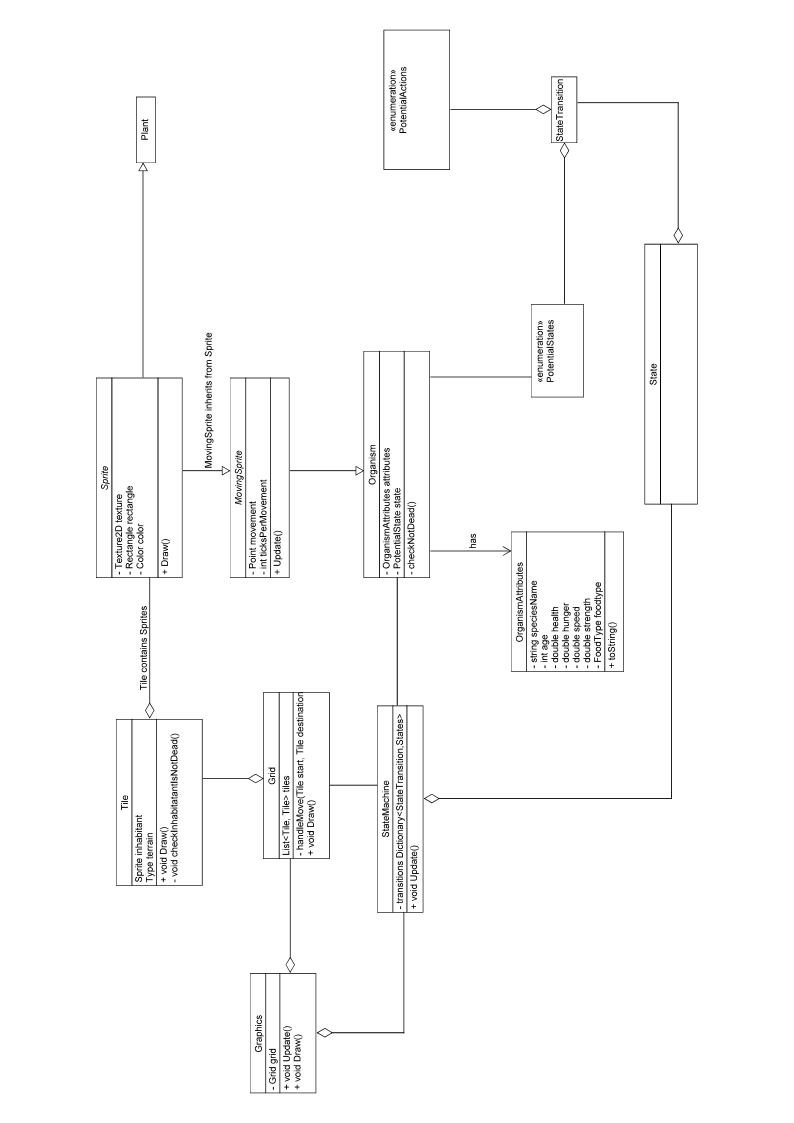
\includegraphics[width=\textwidth,height=\textheight]{class-diagram}
\end{figure}

\bibliographystyle{apalike}
\bibliography{references.bib}
	
\end{document}